\ylDisplay{Näiv kujutis} % Ülesande nimi
{EFO žürii} % Autor
{piirkonnavoor} % Voor
{2019} % Aasta
{P 8} % Ülesande nr.
{3} % Raskustase
{
% Teema: Valgusõpetus
\ifStatement
Punktvalgusallikas asub läätse optilisel peateljel nii, et tekkinud näiv kujutis asub läätsele kaks korda lähemal kui valgusallikas. Leidke konstrueerimise teel läätse fookus.
\fi
\ifHint
Kuna lääts tekitab näiva kujutise, mis asub läätsele lähemal kui ese, peab olema tegemist nõgusläätsega. Seega tuleb punktvalgusallika kiirtekäik konstrueerida vastavalt nõgusläätse seaduspärasustele.
\fi
\ifSolution
Kuna lääts tekitab näiva kujutise, mis asub läätsele lähemal kui ese, peab olema tegemist nõgusläätsega. Kuna ese asub optilisel peateljel, siis saame leida kujutise asukoha konstrueerides abikiired. Kõigepealt märgime optilisele peateljele eseme ning kujutise täpselt läätse ja eseme vahele. Tõmbame esemest suvalise kiire läätseni ning selle kiirega paralleelse kiire läbi läätse keskpunkti. Nõguslääts hajutab kiired nii, et kiirte pikendused kohtuvad fokaaltasandil (joonisel punkt $B$). Kuna fokaaltasand läbib eseme $A$ asukohta, siis asub ka fookus punktis $A$.
\begin{center}
	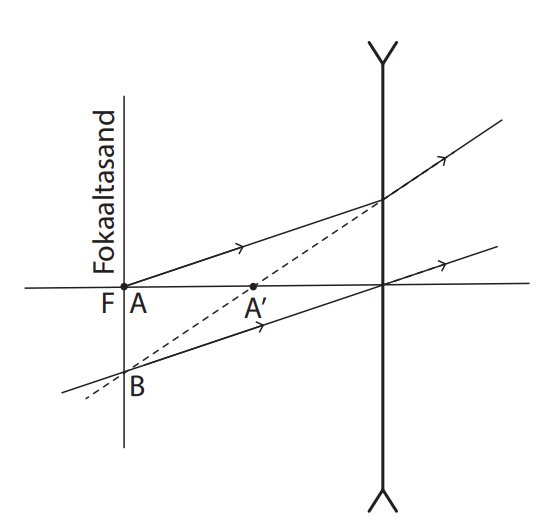
\includegraphics[width=0.5\linewidth]{2019-v2p-08-lah.PNG}
\end{center}
\fi
}
